\section{序論}

\subsection{共有視野保証の重要性と背景}

マルチロボットシステムでは,各ロボットがセンサ情報や視界を共有することにより,監視・捜索・協調輸送などのタスクを効率的に遂行できることが知られている.
特にカメラを用いた視覚協調の場合,各ロボットの共有視野(Common Field-of-View, CoFoV)が不可欠である.例えば,複数ドローンが異なる角度から同一対象を観測できることや,通信の見通し線(LOS)維持が求められる\cite{Panagou2017}.

マルチエージェントVSLAM(Visual Simultaneous Localization and Mapping)においては,各エージェントが撮影した画像から抽出される局所特徴に基づき自己局在を行い,エージェント間で特徴マッチングにより相対位置を推定する.従来のORBやSIFTに代わり,SuperPointのような学習型局所特徴検出・記述器\cite{DeTone2018}や,NetVLADによるグローバル記述子\cite{Arandjelovic2016}が高いロバスト性を示し,ループ検出やキーフレームマッチングに貢献している.

画像特徴量のマッチングを成功させるためには,各エージェントが共通のランドマークを観測できるよう,カメラの視野錐台の幾何学的重複が必要である.視野重複が存在すれば,エージェント間でのループ検出が可能となり,その結果として各ロボットの地図統合が実現される\cite{Zhang2022}.しかし,ロボットは視野角が限られているため,視界共有を保証するための制御技術の開発が急務である.

\red{モチベーション:CoVINSではsuperpoint特徴量などの画像特徴量のマッチングにより、自己位置推定に関する最適化問題のfactorを得ている。特徴量をマッチングするにはエージェントの視野錐台が重なっている必要がある。single agent問題に関してはstereo cameraの相対位置をconstかつgivenとして最適化問題に組み込み、multi agent問題に関しては視野錐台のoverrideは不可知であるために画像全体特徴量の類似度の一致などによってpassiveなevent trigger型としてアルゴリズムが構築されている。しかし、agent1とagent2が視野錐台を交差させ続けるための制御則(CBF等)に基づいてactive perceptionを行う場合、multi agentの自己位置推定においてinter-agentな特徴量のマッチング及び推定問題はエージェントをまたいだカメラ間の相対位置をgiven, もしくは最適化すべき双対変数として複数のエージェント位置を同時最適化できるはずである。さらに、active perceptionの枠組みで考えれば、CBFを用いた最適制御問題と自己位置推定問題も同一の目的関数の最小化問題として扱うことができるはずである。  
上記の仮定から、本セミナーではその手始めとして,代表的なCoVINSであるUAVを対象として、視野錐台を交差させ続けるための分散型CBF手法を提案する。}

\subsection{既存研究の課題}

従来はポテンシャル場やMPC(Model Predictive Control)を用いた手法が提案され,局所的な視界制約下での隊列制御やセンサグラフの連結性維持に取り組まれてきた\cite{Sabattini2013}.一方で,制御バリア関数(Control Barrier Function, CBF)を用いた手法は,制約違反を防ぎながらリアルタイムに最適な制御入力を計算できるため,有力な候補となる\cite{Capelli2020}.

しかし,現状の協調SLAMは,キーフレームの受動的な共有と画像類似度評価に依存しており,視野重複が偶発的に発生しなければマップ統合が成立しないリスクがある.また,多数のロボットを対象とする場合,中央集権的な制御は通信負荷や計算量の面で現実的ではなく,各エージェントが局所的に計算し,限定的な通信で連携する分散アルゴリズムの設計が必要である.

従来の視野維持手法は,対象が視野内にあるか否かを決定論的に評価するに留まっていたが,センサの観測不確実性を十分に取り入れていなかった\cite{Panagou2012}.また,従来の多くの視野制約付き制御手法は,単純な動力学モデル(例:Dubins車両やクアッドロータの水平姿勢維持)に基づいており,非ホロノミックなダイナミクスを明示的に考慮していなかった\cite{Dias2016}.

\subsection{本研究の貢献}

本研究では,SE(3)上における協調自己位置推定のための視野共有を保証する分散型CBF手法を提案する.本研究の主な貢献は以下の通りである.

\begin{itemize}
\item SE(3)における共有視野保証を実現する.従来のステレオ視やリーダーフォロワ形式による視野制御は,ロボット間の相対配置を幾何学的に制約するに留まっていたが,本手法は3次元空間におけるエージェント全体の姿勢・位置を統合的に制御する枠組みを提供する.

\item 特徴点に基づく確率的可視性制約とCBFの適用を行う.本研究では,各エージェントが観測する特徴点に基づき,その可視性を確率的に評価した上で,CBFに組み込み,常時高い確率で共有視野が確保されるよう制御入力を設計する.これにより,センサノイズ等による不確実性下でも安全な視野維持が可能となる.

\item 非ホロノミックなドローンダイナミクスへの対応と分散最適化を実現する.本研究では,機体の並進および回転運動を同時に考慮するSE(3)上の非ホロノミックドローンモデルに対して,高次制約も扱える高次制御バリア関数(HOCBF)を導入し,各エージェントが局所的な情報交換を通じて分散最適化アルゴリズム(PDMM等)により制御解を求める枠組みを提案する\cite{Lv2024}.これにより,リアルタイム性とスケーラビリティの両立を実現する.
\end{itemize}

\subsection{論文構成}

本論文の構成は以下の通りである.第2章ではCBFの基本概念と高次CBFについて説明する.第3章では問題設定とシステムモデルについて述べる.第4章では共有視野のためのCBFを提案し,第5章では二次系システムのための高次CBFを導入する.第6章ではシミュレーション結果を示し,第7章で結論と今後の課題について述べる.

\begin{figure}[htbp]
\centering
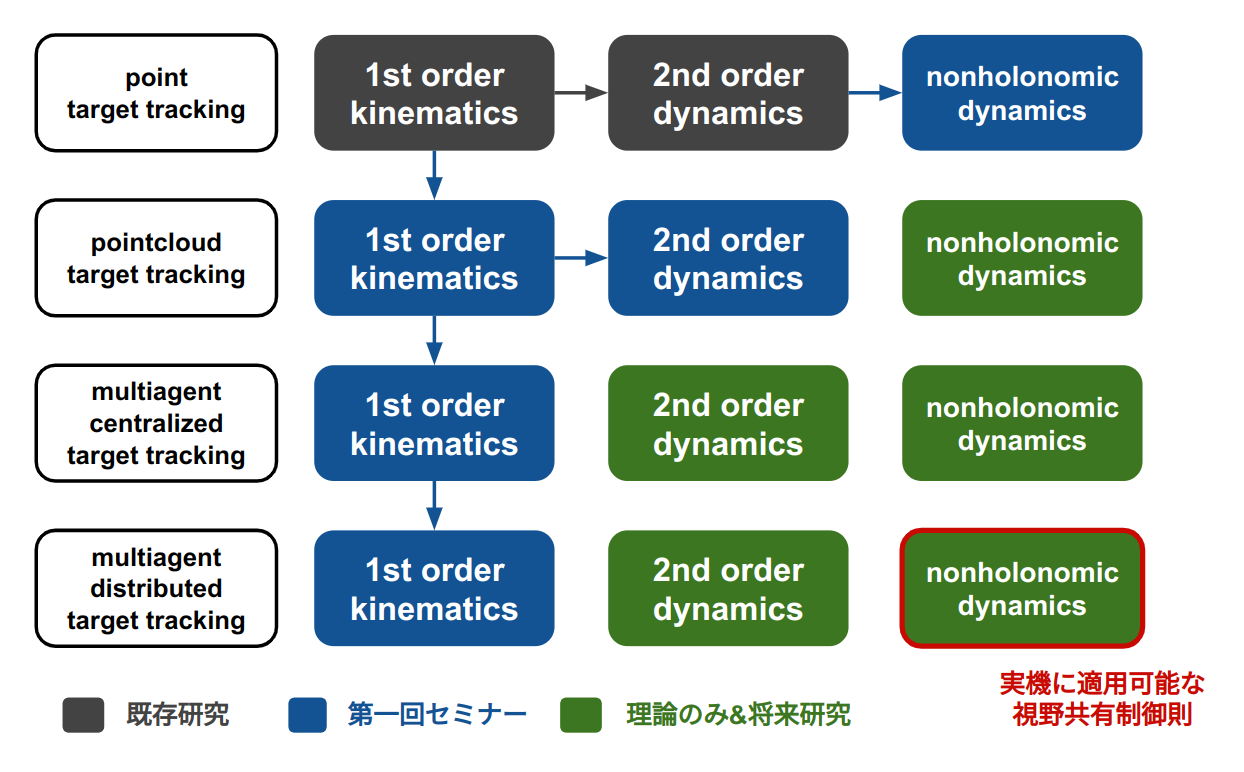
\includegraphics[width=0.8\linewidth]{fig/progress.png}
\caption{第一回セミナーの内容と本研究の貢献点}
\label{fig:progress}
\end{figure}